% !TEX root = poster.tex
\headerbox{\textbf{Flavour Tagging in Run I}}{name=run1,column=1,span=2,row=0}{
\begin{minipage}{0.474\boxwidth}
\textbf{Handling for analyses}\\[-0.85em]
\begin{itemize}
\setlength\itemsep{0.01em}
\vspace{-0.3em}
\item one calibration per tagger valid for all channels
\item systematic uncertainties from
\begin{itemize}
\setlength\itemsep{0.01em}
\setlength{\itemindent}{-.11in}
\vspace{-0.4em}
\item[${\color{tu_gruen}-}$] calibration methods
\item[${\color{tu_gruen}-}$] results in different control channels 
\end{itemize}
\vspace{-0.4em}
\item "ad-hoc" calibration from specific control channels for analyses dominated by FT uncertainty %(\BdToJPsiKS)
\end{itemize}
\vspace{-0.9em}
%\begin{center}
%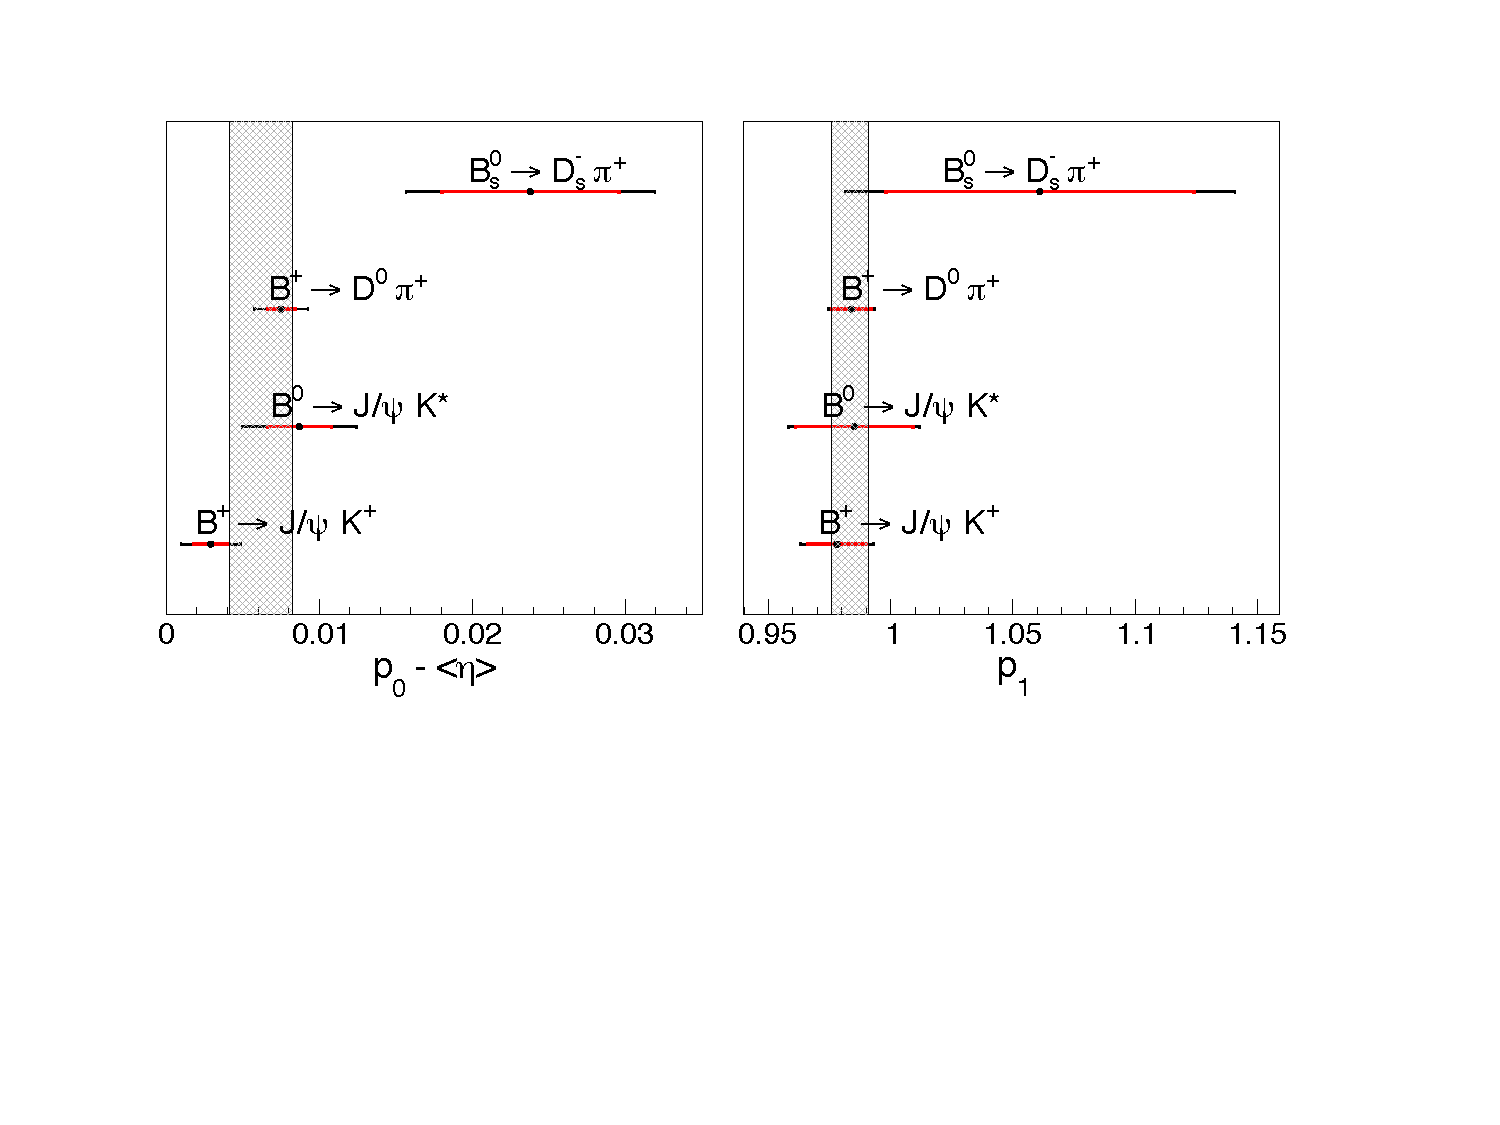
\includegraphics[width=0.466\boxwidth]{graphP0P1.pdf}
%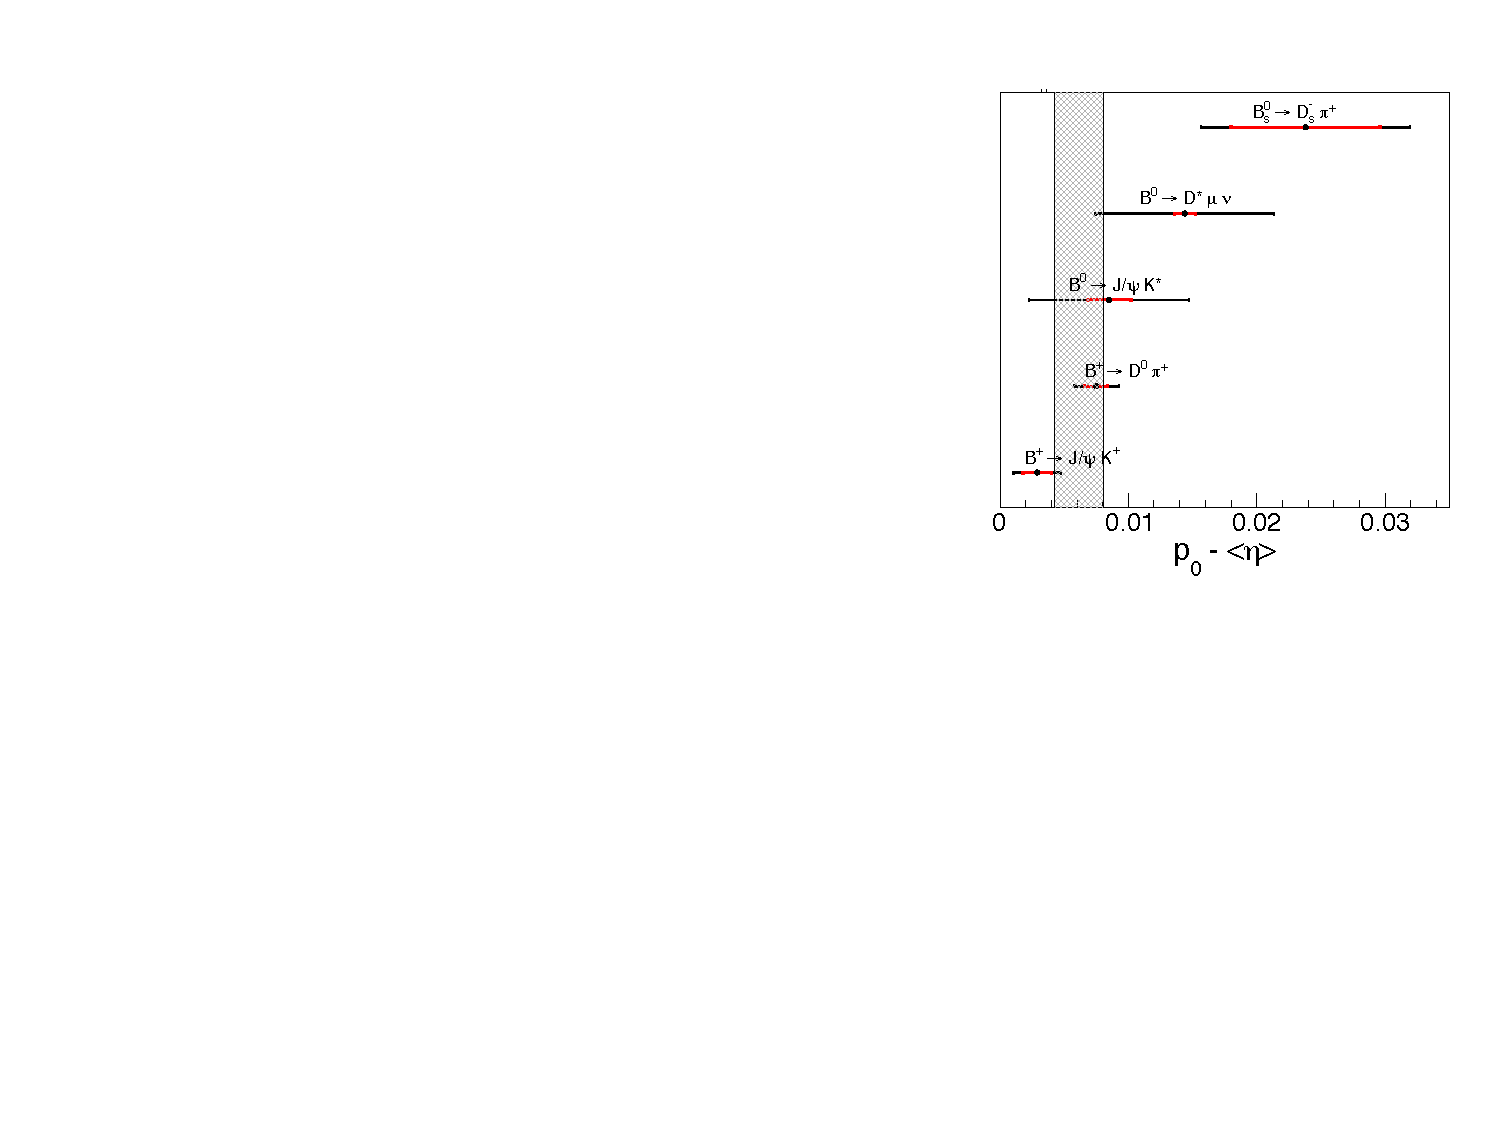
\includegraphics[width=0.233\boxwidth]{portability_p0.pdf}
%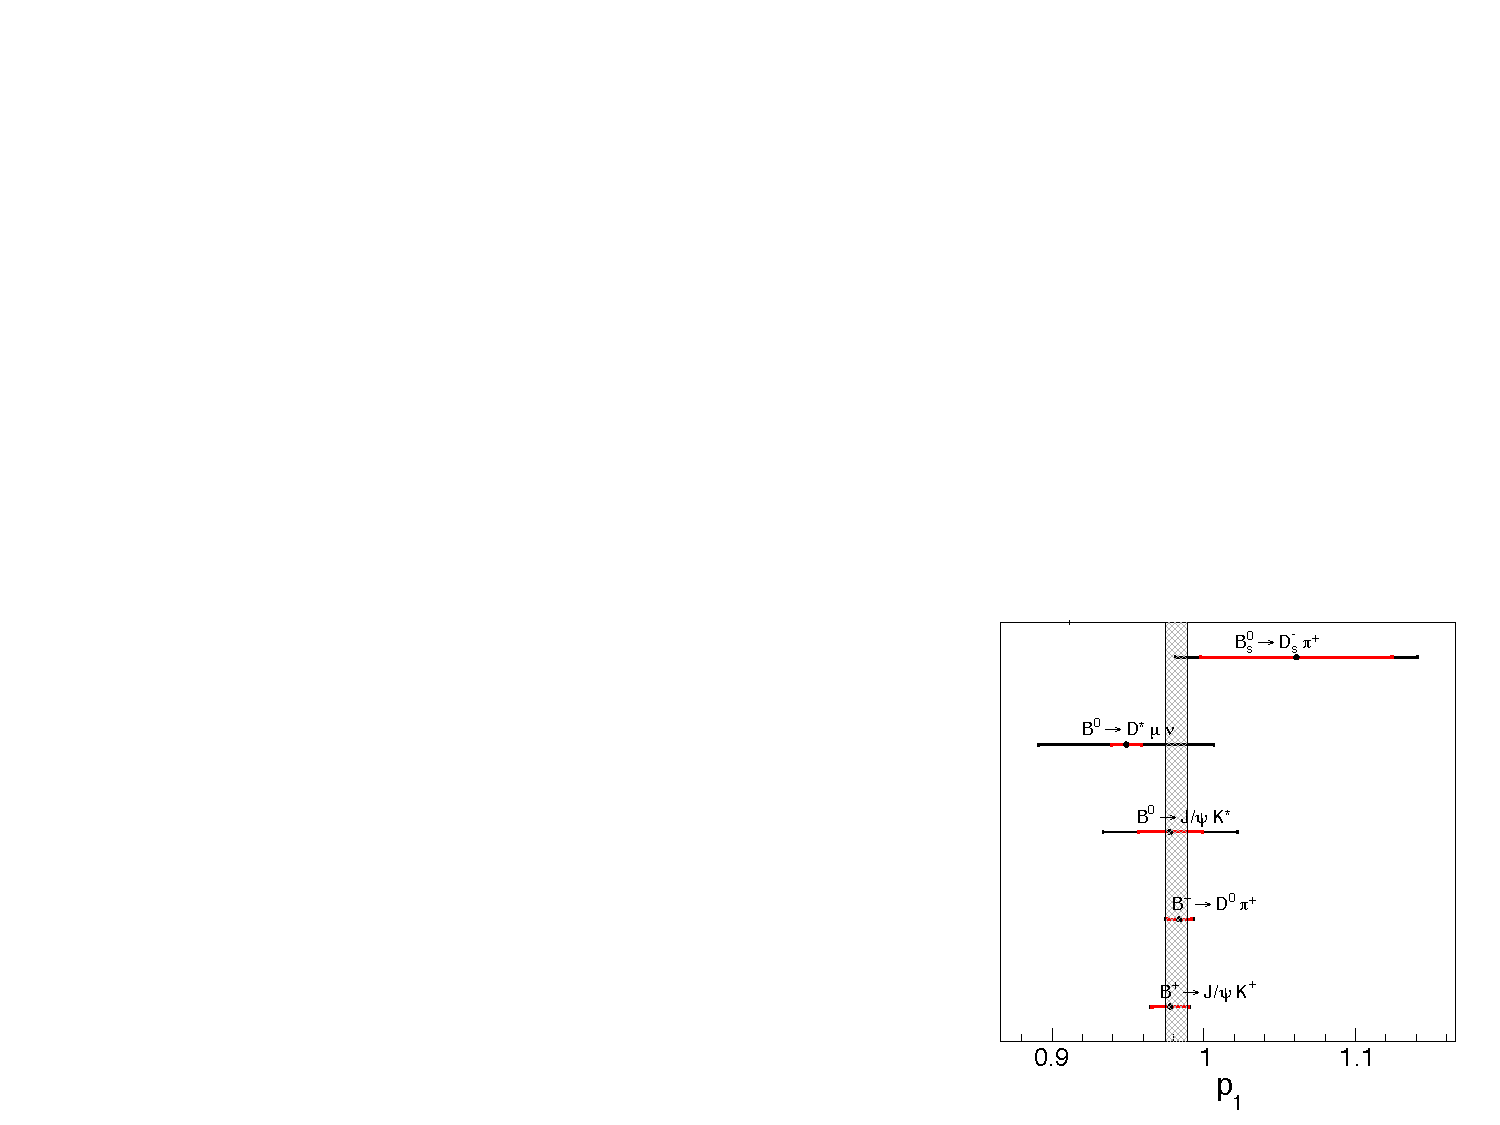
\includegraphics[width=0.233\boxwidth]{portability_p1.pdf}
%\end{center}
\vspace{1.05em}
\textbf{Highlights of successful FT uses}
\vspace{-0.5em}
\begin{itemize}
\item\textbf{\CP violation in \BsToJPsipipi}

\vspace{-1.7em}
\begin{center}
\includegraphics[width=0.315\boxwidth]{figures/Jpsipipi_SSK.pdf}
\end{center}
\vspace{-2.7em}

	\begin{itemize}
	\setlength\itemsep{0.01em}
	\setlength{\itemindent}{-.11in}
	\item[${\color{tu_gruen}-}$] analysis on \num{2011} data: $\varepsilon_\text{eff}=\SI{2.43}{\%}$ [3] 
	\item[${\color{tu_gruen}-}$] full Run I analysis: $\varepsilon_\text{eff}=\SI{3.89}{\%}$ [4] 
	\item[${\color{tu_gruen}-}$] newest analysis profited from 
	\setlength{\itemindent}{.05in}
	\item[${\color{tu_gruen}\rightarrow}$] including SS kaon nnet tagger
	\item[${\color{tu_gruen}\rightarrow}$] re-optimisation of OS algorithms
	\end{itemize}
	
\item\textbf{\CP violation in \BsToDsK}

\vspace{-2.1em}
\begin{flushleft}
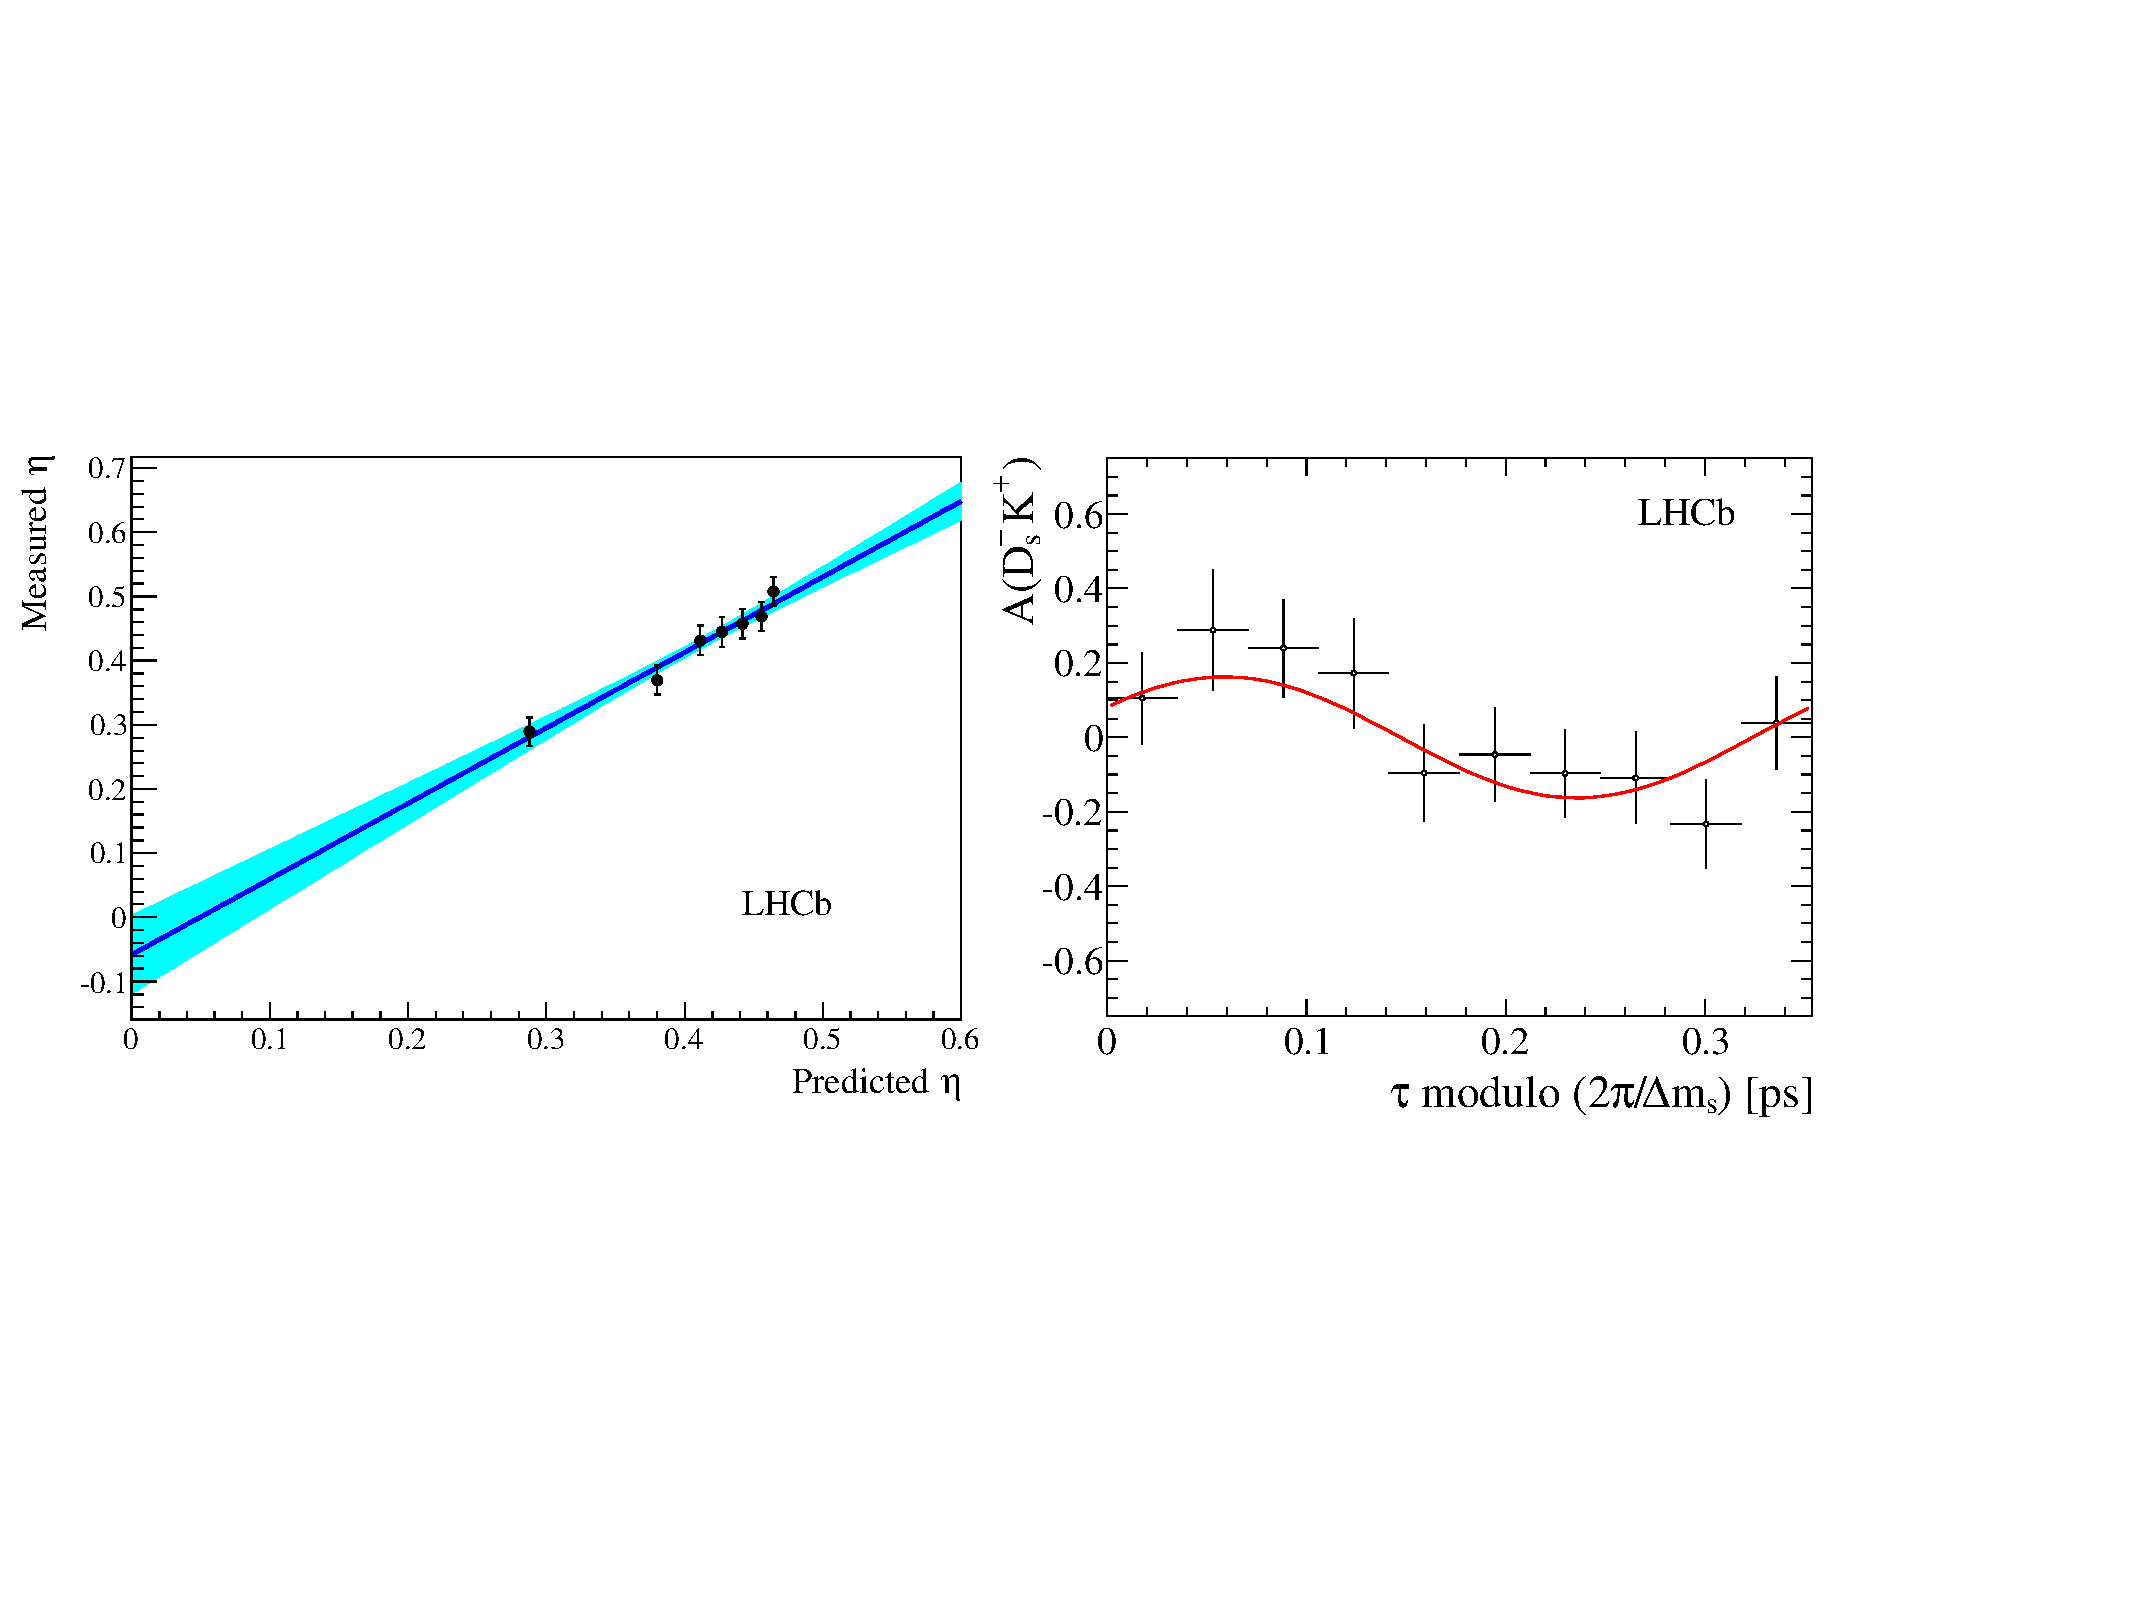
\includegraphics[width=0.474\boxwidth]{CPV_DsK2.pdf}
\end{flushleft}
\vspace{-2.8em}

	\begin{itemize}
	\setlength\itemsep{0.01em}
	\setlength{\itemindent}{-.11in}
	\item[${\color{tu_gruen}-}$] analysis on \num{2011} data: to $\varepsilon_\text{eff}=\SI{5.07}{\%}$
	\item[${\color{tu_gruen}-}$] SS kaon nnet adds more than \SI{1.3}{\%} to $\varepsilon_\text{eff}$ [5]
	\end{itemize}
\end{itemize}
\end{minipage}
\vspace{0.7em}
\hfill
\begin{minipage}{0.474\boxwidth}
\vspace{-0.2em}
\begin{itemize}
\item\textbf{\CP violation in \BdToJPsiKS ($\sin2\beta$)}
	\begin{itemize}
	\setlength\itemsep{0.01em}
	\setlength{\itemindent}{-.11in}
	\item[${\color{tu_gruen}-}$] analysis on \num{2011} data: $\varepsilon_\text{eff}=\SI{2.38}{\%}$ [6]
	\item[${\color{tu_gruen}-}$] full Run I analysis: $\varepsilon_\text{eff}=\SI{3.02}{\%}$ [7] 
	\setlength{\itemindent}{.05in} 
	\item[${\color{tu_gruen}\rightarrow}$] SS pion tagger adds more than \SI{0.376}{\%} to $\varepsilon_\text{eff}$ 
	\end{itemize}
	
\vspace{-1.7em}
\begin{center}
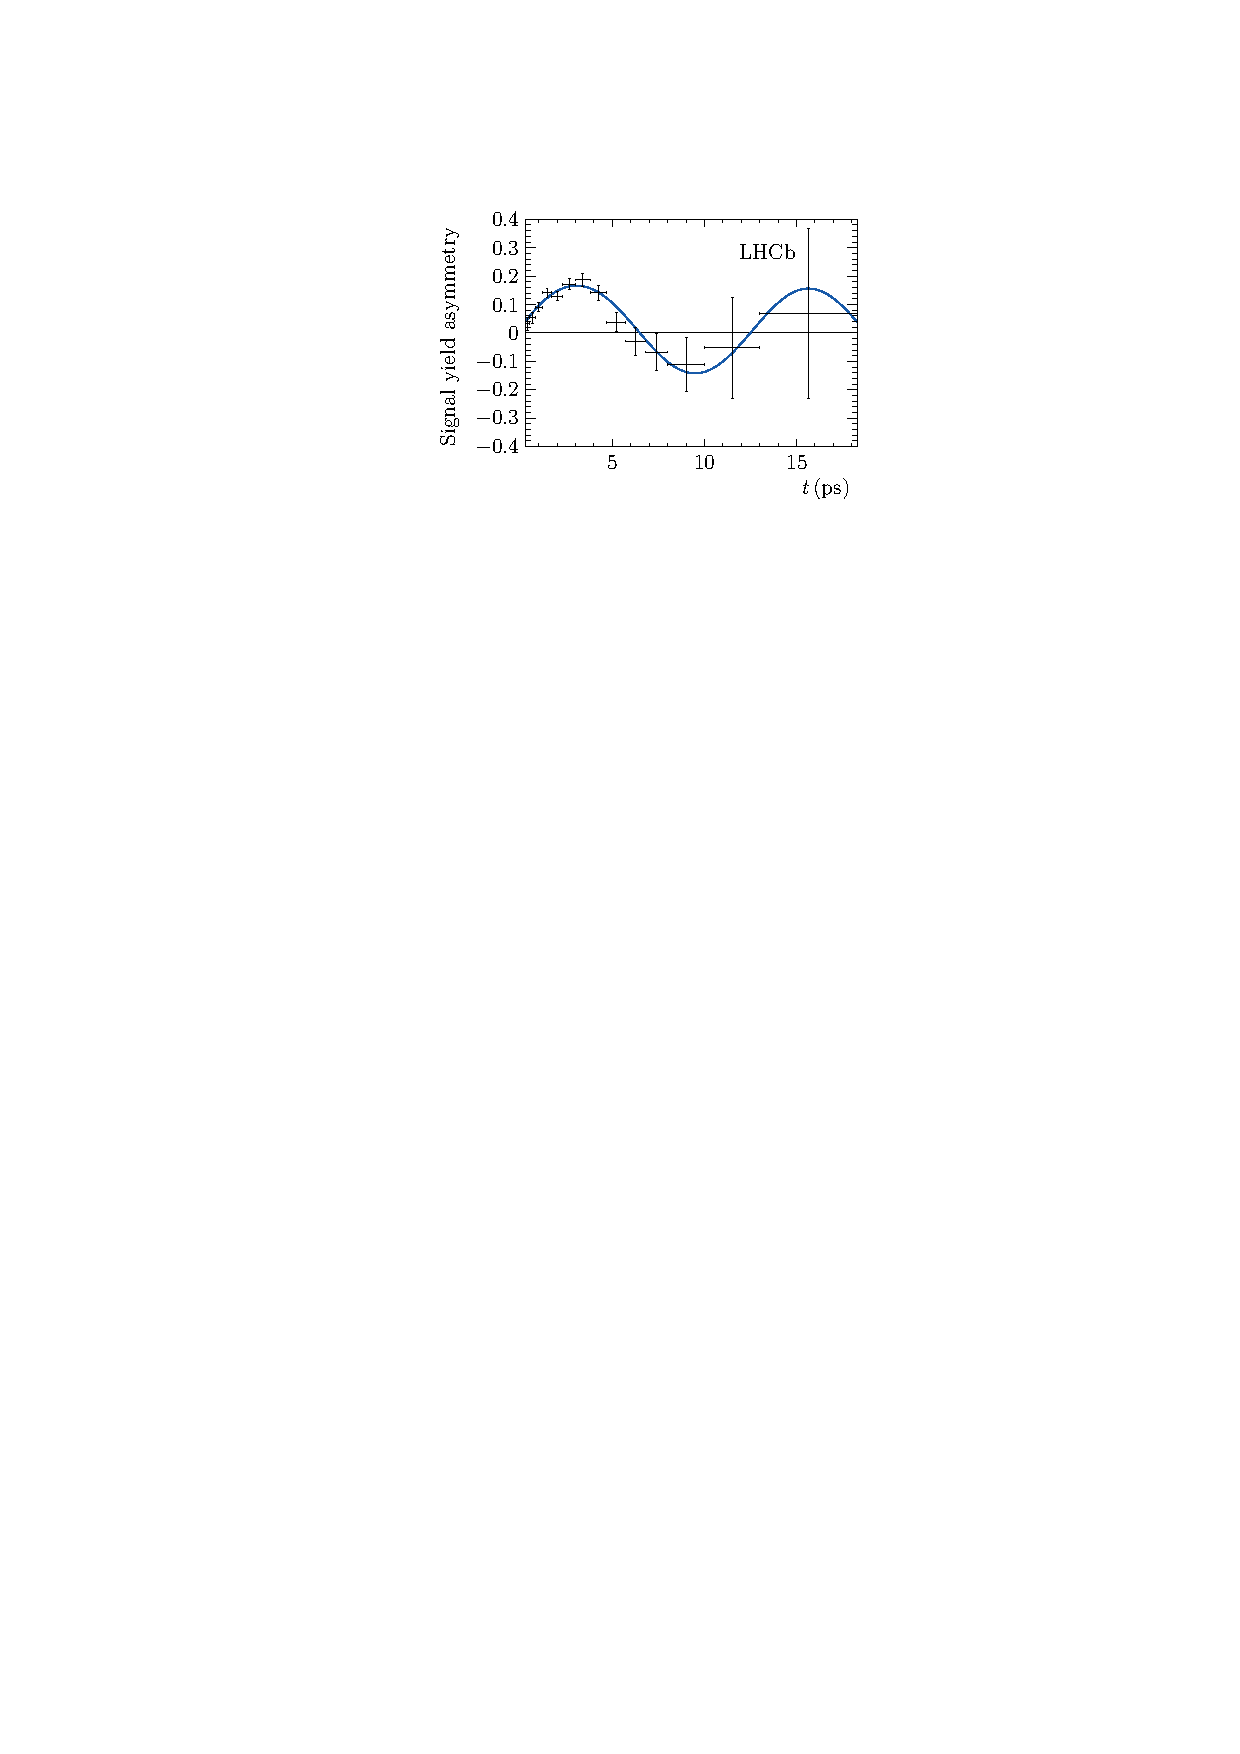
\includegraphics[width=0.315\boxwidth]{CPV_sin2beta.pdf}
\end{center}
\vspace{-2.5em}

	\begin{itemize}
	\setlength{\itemindent}{-.11in}
	\setlength\itemsep{0.01em}
	\item[${\color{tu_gruen}-}$] precision analysis \hspace{0.1em}${\color{tu_gruen}\rightarrow}$ "ad-hoc" calibration
	\setlength{\itemindent}{.05in}
	%\item[${\color{tu_gruen}\rightarrow}$] smaller uncertainties from FT 
	\item[${\color{tu_gruen}\rightarrow}$] OS algorithms calibrated with \BuToJPsiKp 
	\item[${\color{tu_gruen}\rightarrow}$] SS pion calibrated with \BdToJPsiKst
	\end{itemize}

%\item\textbf{\BsTophiphi}

\item\textbf{\CP violation in \BsToJPsiKS}
	\begin{itemize}
	\setlength\itemsep{0.01em}
	\setlength{\itemindent}{-.11in}
	%\item[${\color{tu_gruen}-}$] \Bs and \Bd events not separable in analysis
	\item[${\color{tu_gruen}-}$] \Bs events: $\varepsilon_\text{eff}=\SI{4.00}{\%}$ [8]
	\item[${\color{tu_gruen}-}$] \Bd events: $\varepsilon_\text{eff}=\SI{2.62}{\%}$ [8]
	\setlength{\itemindent}{.05in}
	\item[${\color{tu_gruen}\rightarrow}$] also small contribution of SS kaon for \Bd
	\item[${\color{tu_gruen}\rightarrow}$] origins of this effect:
	\setlength{\itemindent}{.10in}
	\item[${\color{tu_gruen}-}$] same-side protons misidentified as kaons
	\item[${\color{tu_gruen}-}$] kaons from same-side \Kstar(892) 
	\setlength{\itemindent}{.05in}
	\item[${\color{tu_gruen}\Rightarrow}$] kaons have opposite charge for \Bd: tagging decision has to be inverted
	\end{itemize}

\vspace{-1.9em}
\begin{center}
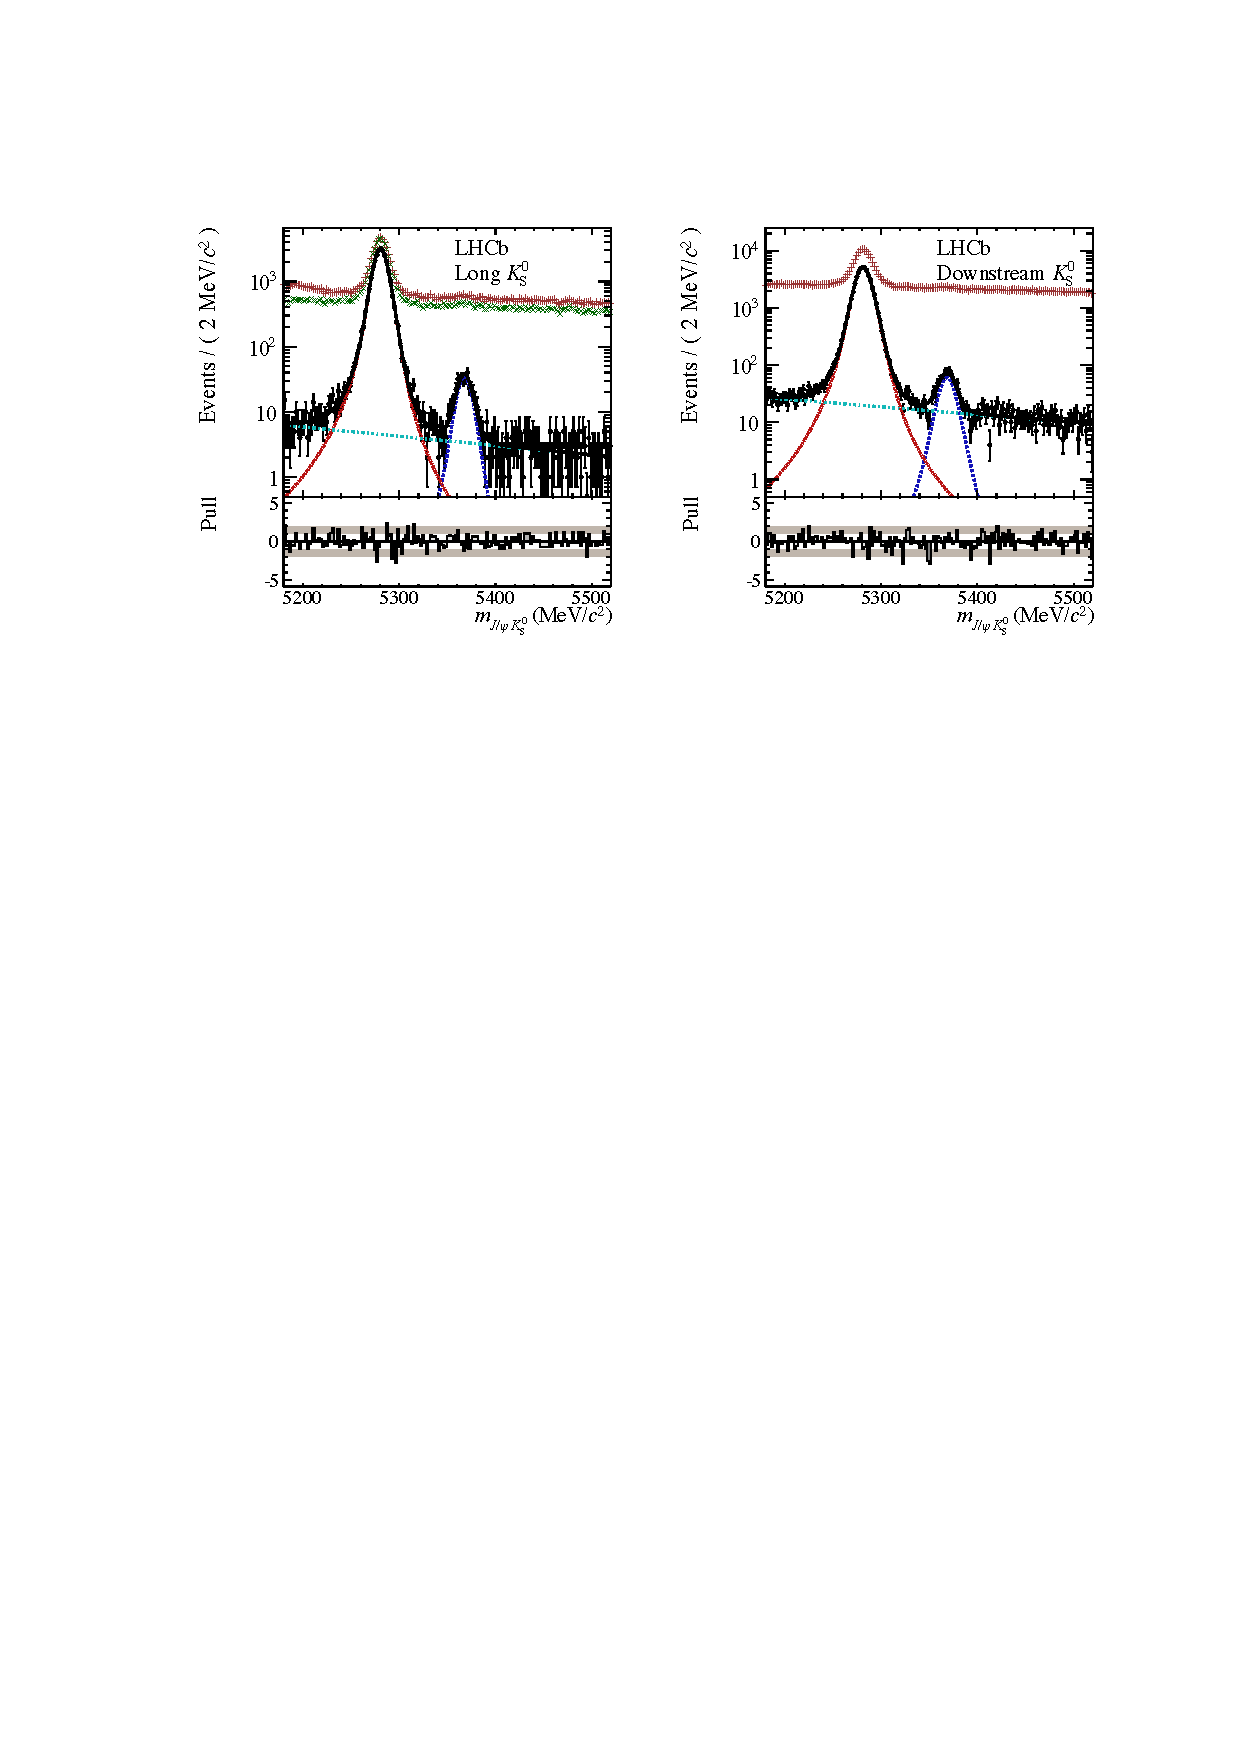
\includegraphics[width=0.43\boxwidth]{CPV_BsJpsiKS.pdf}
\end{center}
%\vspace{-2.4em}
%\item\textbf{Measurement of \dms with \BsToDspi}
%
%\vspace{-1.7em}
%\begin{center}
%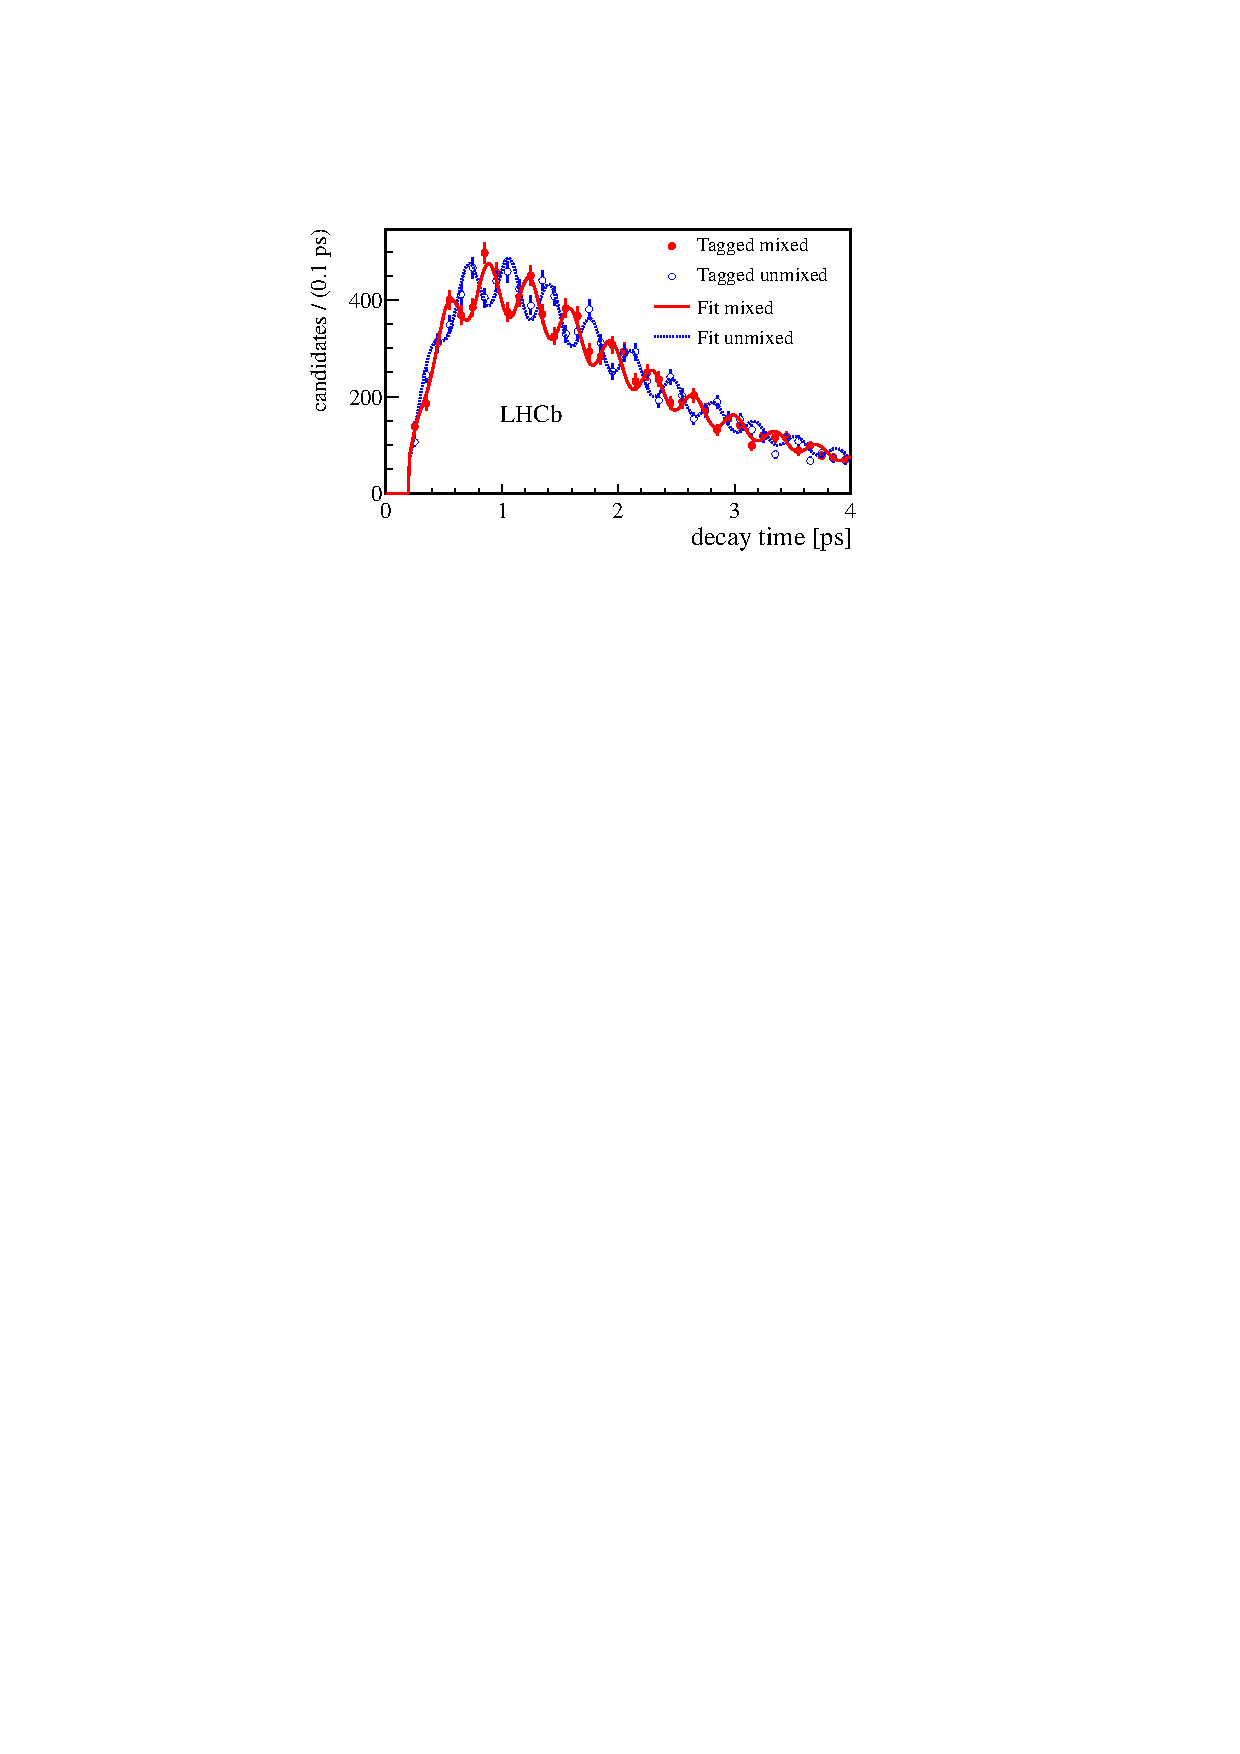
\includegraphics[width=0.266\boxwidth]{Bs_mixing1.pdf}
%\end{center}
%\vspace{-2.5em}
%
%	\begin{itemize}
%	\item[${\color{tu_gruen}-}$] Decay rates: $e^{-\Gamma t}\left(...+\!d\cos\left(\Delta mt\right)\right)$
%	\end{itemize}
\end{itemize}

%\textbf{Overall performance improvements in Run I}
%\begin{itemize}
%\setlength\itemsep{0.01em}
%\vspace{-0.3em}
%\item OS tagging improved $\mathcal{O}$(15\%) 
%\item SS kaon tagging improved $\mathcal{O}$(40\%)
%\vspace{0.5em}
%\setlength{\itemindent}{.14in}
%\item[$\color{tu_gruen}\Rightarrow$] \textbf{Flavour Tagging has been a success in Run I}
%\end{itemize}
\end{minipage}
\vspace{-0.5em}
}
